\chapter{Literature Review}
\label{chap:literature_review}

\section{Introduction}
\label{sec:lit_review_intro}

Depth estimation involves the process of predicting the distance of objects within a scene from a specific camera's perspective. Before the advent of machine learning, this field primarily relied on geometric and optical techniques. This chapter will review both the traditional methods and the modern approaches based on machine learning.

\begin{figure}[htbp!]
    \centering
    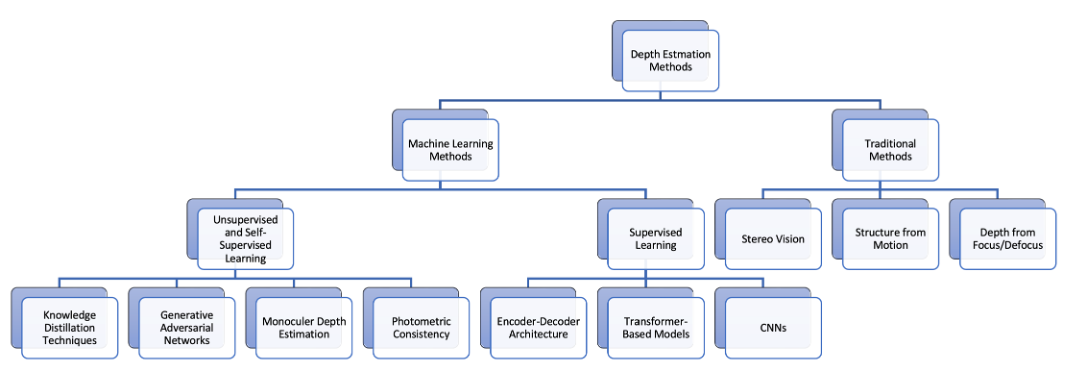
\includegraphics[width=\textwidth]{images/flowchart.png}
    \caption{Methods of Depth Estimation.}
    \label{fig:depth_methods_flowchart}
\end{figure}

\section{Traditional Methods}
\label{sec:traditional_methods}

Traditional methods relied on geometric principles to infer depth. The most important of these are:

\begin{itemize}
    \item \textbf{Stereo Vision:} This technique uses two or more cameras to capture images from slightly different viewpoints and then calculates a depth map through triangulation, as shown in figure \ref{fig:stereo_vision_diagram}. This method requires precise calibration and faces difficulties in textureless regions \cite{scharstein2002taxonomy}.
    
    \begin{figure}[htbp!]
        \centering
        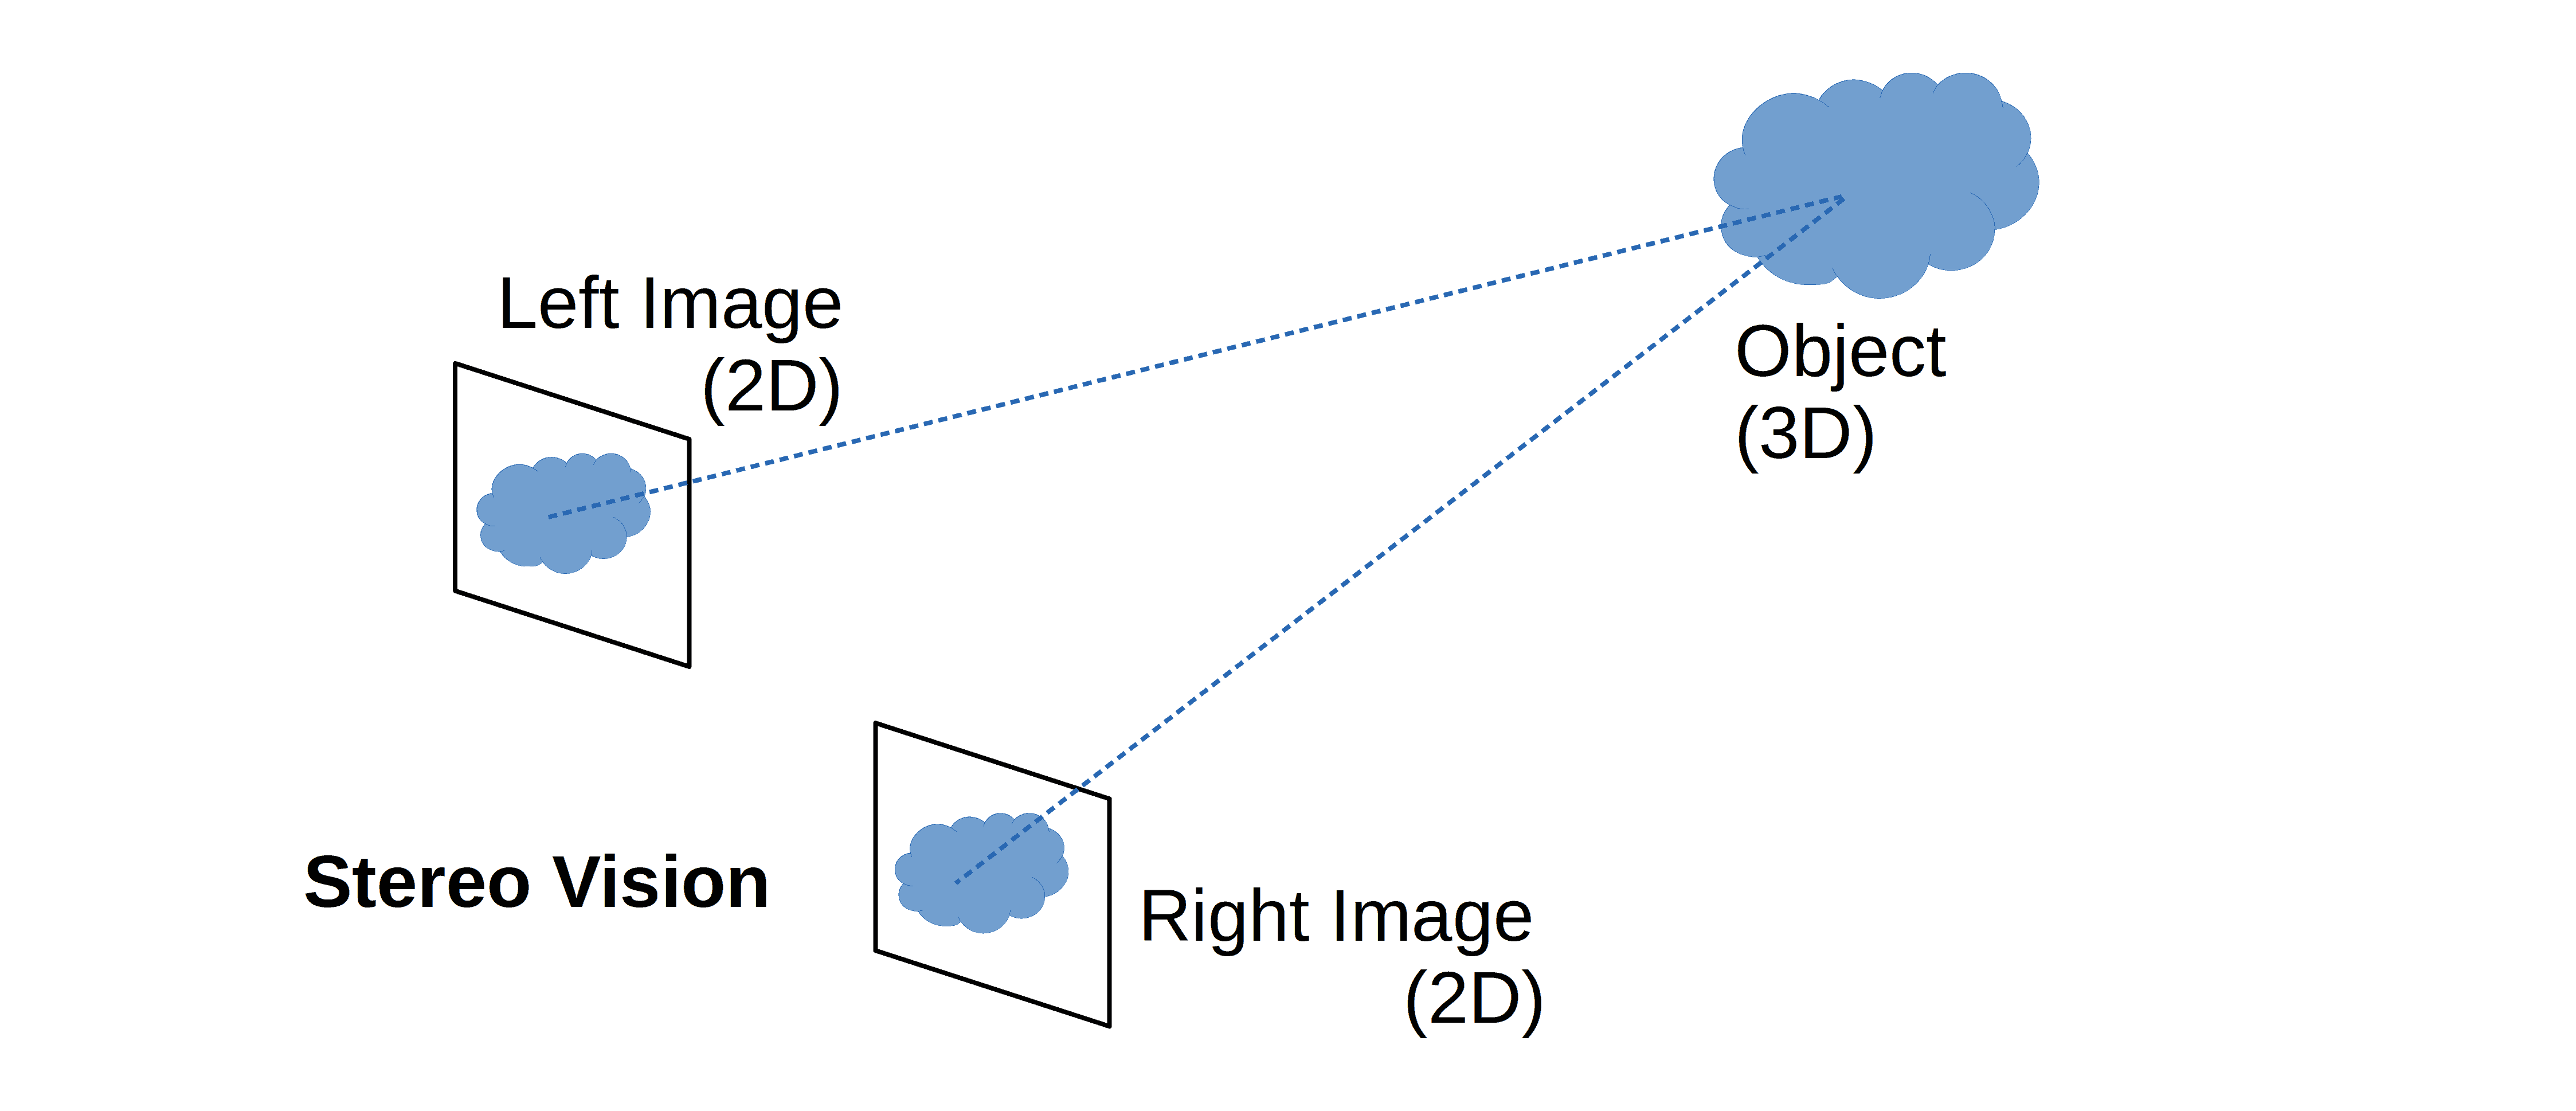
\includegraphics[width=0.8\textwidth]{images/stereo_vision.png}
        \caption{Stereo Vision.}
        \label{fig:stereo_vision_diagram}
    \end{figure}

    \item \textbf{Structure from Motion (SfM):} SfM estimates depth by analyzing the movement of distinctive points across a series of images, which allows for the reconstruction of the scene's 3D structure, demonstrated in figure \ref{fig:sfm_diagram}. This method is sensitive to tracking errors and is computationally expensive \cite{hartley2003multiple,saxena20083}.
    
    \begin{figure}[htbp!]
        \centering
        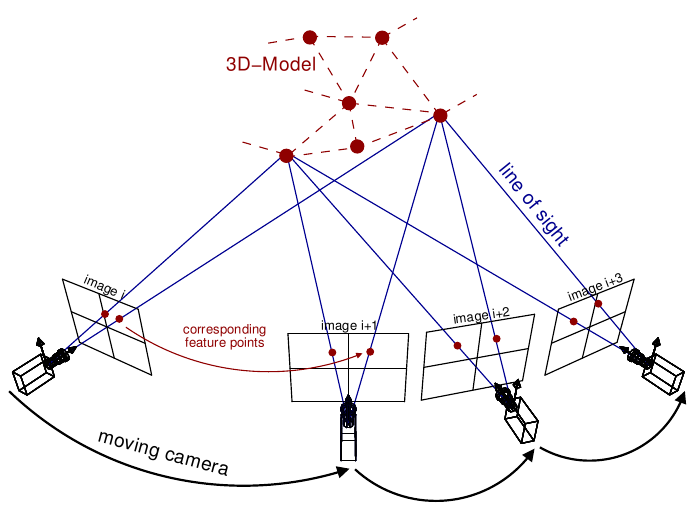
\includegraphics[width=0.9\textwidth]{images/sfm_diagram.png}
        \caption{Structure from Motion.}
        \label{fig:sfm_diagram}
    \end{figure}

    \item \textbf{Depth from Focus/Defocus:} This technique estimates depth based on the degree of blur (defocus) in an image at different focal lengths, as shown in figure \ref{fig:dfd_diagram}. However, this method requires controllable lighting conditions and is limited to the camera's depth of field \cite{pentland1987new}.
    
    \begin{figure}[htbp!]
        \centering
        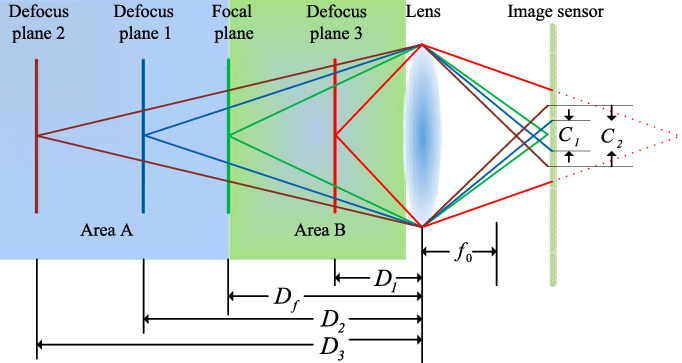
\includegraphics[width=\textwidth]{images/dfd_diagram.png}
        \caption{Depth from Focus/Defocus.}
        \label{fig:dfd_diagram}
    \end{figure}
\end{itemize}

\section{Machine Learning Methods}
\label{sec:deep_learning_methods}

Machine learning models, especially deep learning, have brought about a paradigm shift in the field. They can be divided into:

\subsection{Supervised Learning}
\label{subsec:supervised}

Supervised learning methods require datasets labeled with ground-truth depth maps. These methods have achieved advanced performance by leveraging large-scale datasets and advanced neural network architectures. Key architectures in this approach include:

\begin{itemize}
    \item \textbf{Convolutional Neural Networks (CNNs):} One of the first deep learning models for depth estimation used a multi-scale CNN to predict depth from a single image \cite{eigen2014depth}. This model demonstrated the potential of deep learning for this task.
    \item \textbf{Encoder-Decoder Architectures:} Architectures like U-Net and its variants are widely used for dense depth prediction. These structures combine high-level semantic features with low-level spatial details to produce accurate depth maps \cite{ronneberger2015u}.
    \item \textbf{Transformer Models:} Recent works have discussed the use of Vision Transformers (ViTs) in depth estimation applications \cite{ranftl2021vision}. Transformers capture global context more effectively than CNNs, leading to improved performance in complex scenes.
    \item \textbf{Foundation Models for Depth Estimation:} Early foundational work like MVSNet, an end-to-end deep learning architecture for inferring depth maps from multi-view images \cite{yao2018mvsnet}. More recent work like Depth Anything combines a ViT-L/DPT architecture with DINOv2 pre-training and an affine-invariant loss, achieving state-of-the-art performance without fine-tuning. Its main innovation lies in scaling up to 62 million unlabeled images via automated pseudo-labeling \cite{yang2024depth}.
\end{itemize}

\subsection{Unsupervised and Self-Supervised Learning}
\label{subsec:unsupervised}

Unsupervised and self-supervised methods do not require ground-truth depth maps, making them more scalable and practical for real-world applications. They rely on concepts such as:

\begin{itemize}
    \item \textbf{Photometric Consistency:} This relies on minimizing the photometric error between the original and predicted images using the predicted depth and camera pose. This approach leverages geometric constraints to train the model without labeled data \cite{godard2017unsupervised}.
    \item \textbf{Generative Adversarial Networks (GANs):} GANs have been used to generate realistic depth maps by learning the data distribution \cite{xu2022unsupervised}. These models can improve the quality of depth predictions through adversarial training.
    \item \textbf{Distillation Techniques:} A pre-trained model is used to produce semi-reliable depth maps, and the target model is trained on them \cite{he2025distill}. The student model is typically smaller than the pre-trained teacher model.
\end{itemize}

\begin{table}[htbp!]
    \centering
    \caption{Traditional VS Machine Learning Methods for Depth Estimation.}
    \label{tab:method_comparison}
    \begin{tabularx}{\textwidth}{l >{\RaggedRight}X >{\RaggedRight\arraybackslash}X}
        \toprule
        \textbf{Criterion} & \textbf{Traditional Methods} & \textbf{Machine Learning} \\
        \midrule
        Accuracy & Good & High (with sufficient training) \\
        \addlinespace
        Data Requirement & No need for training data & Requires huge amounts of labeled data for supervised learning and unlabeled data for unsupervised ones \\
        \addlinespace
        Speed & Generally slow but can be real-time & Faster than traditional methods, but requires computational resource \\
        & (e.g., Stereo Vision) & \\
        \bottomrule
    \end{tabularx}
\end{table}

\section{Evaluation Metrics}
\label{sec:evaluation_metrics}
The performance of depth estimation models is evaluated using a variety of metrics, including \cite{gurram2023metrics}:
\begin{itemize}
    \item \textbf{Absolute Relative Difference (Abs Rel):} Measures the relative difference between the predicted and ground-truth depth.
    \item \textbf{Squared Relative Difference (Sq Rel):} Measures the square of the relative difference, emphasizing larger errors.
    \item \textbf{Root Mean Squared Error (RMSE):} Calculates the square root of the average of squared differences.
    \item \textbf{Scale-Invariant Logarithmic Error (SILog):} Accounts for the scale ambiguity in monocular depth estimation, where we know the relative depth between objects but not the absolute metric depth.
    \item \textbf{Accuracy Threshold ($\delta$):} The percentage of pixels where the predicted depth is within a certain threshold of the ground-truth depth, such as $\delta < 1.25$.
\end{itemize}

\section{Datasets for Depth Estimation}
\label{sec:datasets}

The availability of high-quality datasets has been crucial for the advancement of depth estimation. Key datasets include:
\begin{itemize}
    \item \textbf{KITTI:} A widely used dataset for autonomous driving \cite{geiger2012we}, providing stereo images and LiDAR-based depth maps.
    \item \textbf{NYU Depth V2:} An indoor dataset captured with a Microsoft Kinect, containing RGB-D images \cite{silberman2012indoor}.
    \item \textbf{Make3D:} An outdoor dataset containing scenes with laser-scanned depth maps \cite{saxena20083}.
    \item \textbf{Cityscapes:} A large-scale dataset for urban scene understanding, which includes depth maps \cite{cordts2016cityscapes}.
    \item \textbf{COCO:} Although primarily for object recognition, its diversity can be leveraged for depth estimation \cite{lin2014microsoft}.
\end{itemize}

\section{Lightweight Neural Network Architectures}
\label{sec:architectures}

Designing lightweight neural networks is a cornerstone of AI applications on mobile and resource-constrained devices. While this report focuses on MobileNetV3 and MobileViT-XS, the field is rich with innovative architectures seeking to balance accuracy and computational efficiency. Reviewing these architectures provides deeper context and highlights the reasons for choosing MobileViT as the final encoder.

\begin{enumerate}
    \item \textbf{The MobileNet Family:} The MobileNet series is one of the most famous architectures designed for mobile devices Its core idea is to replace costly traditional convolutions with Depthwise Separable Convolutions. This change significantly reduces the number of parameters and computational operations. MobileNetV3 was considered at the beginning of this project, as this version offers further improvements through architectures enhanced by Neural Architecture Search (NAS) and attention mechanisms (Squeeze-and-Excite) \cite{koonce2021mobilenetv3}.
    \item \textbf{The EfficientNet Architecture:} This introduced a new model scaling approach known as Compound Scaling. Instead of arbitrarily scaling one network dimension (like depth or width), EfficientNet uniformly scales all dimensions (depth, width, and image resolution) in a principled manner. This approach allowed it to achieve superior accuracy with significantly fewer parameters compared to its predecessors \cite{koonce2021efficientnet}.
    \item \textbf{The MobileViT Architecture:} Vision Transformers (ViT) have demonstrated superior ability to capture global context thanks to the self-attention mechanism, but they come at a huge computational cost, making them unsuitable for mobile phones. Herein lies the true strength of MobileViT; it is not just a convolutional or transformer architecture, but a hybrid that combines the best of both worlds \cite{mehta2021mobilevit}:
    \begin{itemize}
        \item \textbf{Local Efficiency of CNNs:} MobileViT uses efficient convolutions in its initial layers to extract local features from the image.
        \item \textbf{Global Capability of Transformers:} It then feeds these local features into lightweight transformer layers specifically designed for mobile phones, allowing the model to understand the relationships between different parts of the image and build a holistic understanding of the scene.
    \end{itemize}
\end{enumerate}

The table \ref{tab:arch_comparison} summarizes the key comparison points between these architectures:

\begin{table}[htbp!]
    \centering
    \caption{Comparison of Lightweight Network Architectures.}
    \label{tab:arch_comparison}

    \begin{tabularx}{\textwidth}{
        >{\bfseries}l 
        >{\RaggedRight}X 
        >{\RaggedRight}X 
        >{\RaggedRight\arraybackslash}X 
    }
        \toprule
        Architecture & Core Principle & Computational Efficiency & Observations from Project Experience \\
        \midrule
        MobileNetV3 & 
        Uses Depthwise Separable Convolutions to reduce computations, with enhancements via NAS and Squeeze-and-Excite mechanisms. &
        Very high; designed to significantly reduce parameters and operations, making it suitable for mobile devices. & 
        Used in initial training attempts, but results were poor as the depth maps lost many fine spatial details. \\
        \addlinespace

        EfficientNet & 
        Adopts "Compound Scaling," which systematically and uniformly scales network depth, width, and resolution. & 
        Extremely efficient, achieving high accuracy with far fewer parameters than preceding models. & 
        Tested, but results were not good for depth estimation. The likely reason is that the architecture focuses on classification and does not preserve the spatial details needed for depth reconstruction. \\
        \addlinespace

        MobileViT & 
        A hybrid architecture combining efficient CNN convolutions for local features and lightweight Transformer layers for global context. &
        Specifically designed to be light, fast, and suitable for mobile phones, while retaining the ability to understand global context via self-attention. & 
        Achieved the best results and was adopted as the final encoder. Its ability to effectively understand global context was what previous attempts lacked. \\
        \bottomrule
    \end{tabularx}
\end{table}